\subsection{HPC与AI和Big Data融合的需求与可能性}
传统HPC同AI、Big Data融合是新的发展趋势,
由此产生新的领域HPDA(High Performance Data Analysis)
\footnote{关于HPDA并没有明确的定义,
多数表述为HPDA = HPC + Big Data,
也有将AI结合即HPDA = HPC + Big Data + AI},
旨在将HPC、Big Data以及AI进行融合产生更大的价值。
他们之间的关系如\cref{hpc_hpda_ai}所示。

\begin{figure}[ht!]
    \centering
    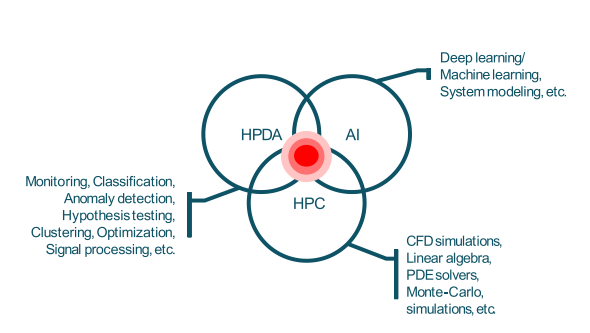
\includegraphics[width=\linewidth]{images/hpc_hpda_ai.png}
    \caption{HPC与HPDA、AI之间的关系}
    \label{hpc_hpda_ai}
\end{figure}

之所以需要并存在这个可能性,主要的原因有\cite{yef2022_hpc}:

\begin{itemize}
    \item 在科学领域,AI for Science出现使得HPC程序中也包含AI算法,
    HPC+AI是刚性需求
    \item 数据处理是AI的基础,数据与AI融合自然高效
    \item HPC本身就存在大数据\footnote{“Do you know what high-performance guys call big data?” … The answer: Data. \cite{hpda_qa}}
    \item HPC、AI、Big Data在基础设施上有着类似的要求,
    如对内存、高性能网络和存储;
    对计算精度的要求上存在差别(HPC要求64位浮点数,AI只需要16位),
    如果能够在一定程度上复用那么在处理器层面可以同时支撑HPC和AI。
    \cref{hpc_vs_hpda}直观反应了传统HPC与HPDA间的差异。
\end{itemize}

\begin{figure}[ht!]
    \centering
    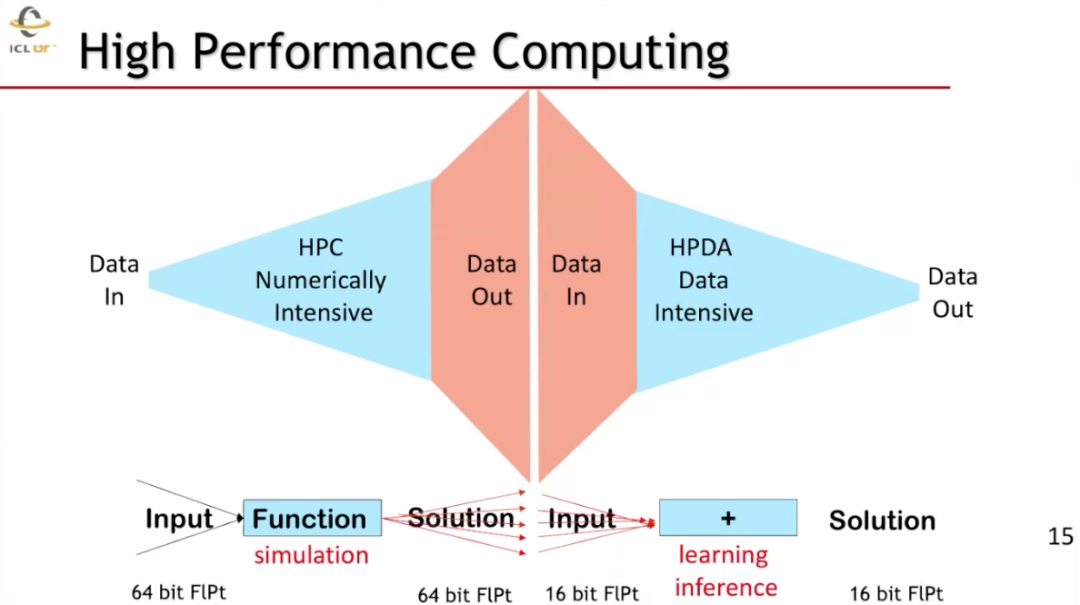
\includegraphics[width=\linewidth]{images/hpc-vs-ai.png}
    \caption{HPC与HPDA的场景对比\cite{jack_hpc_ai}}
    \label{hpc_vs_hpda}
\end{figure}

HPDA的一个应用场景是将科研仿真和AI计算可以非常有效地进行联合,
因为二者都需要模型和数据。
通常,仿真使用(数学)模型产生数据,
(AI)分析使用数据来生成模型。
使用分析方法得到的模型和其他的模型一起可以被用到仿真中去;
仿真产生的数据和其他来源的数据一起可以被用于分析。
这样就形成了一个相互促进的良性循环\cite{jack_hpc_ai}。

在应用HPDA时,可以根据需要组合不同的形式的计算,
从而能够端到端在一个系统内完成功能,
例如使用Sprak对数据进行预处理,使用MPI+TenserFlow来训练模型等。

\subsection{HPDA融合存在的挑战}

HPDA目前处于较为前沿的阶段,
尽管HPC、AI、Big Data等都发展了几十年近乎成熟,
要应用HPDA仍然存在诸多的挑战,
主要有:

\begin{itemize}
    \item 技术栈不兼容,例如编程语言、框架等,
    相互之间存在较大的差别(参见\cref{hpc_bigdata_ai_envs}),
    比如大数据使用的Spark、Hadoop等无法在HPC上使用\cite{hpda_qa}
    \item 需要通用的计算架构,已经有一些将它们融合的尝试,
    例如将Spark应用在HPC上\cite{spark_on_hpc},但是缺乏通用性,且扩展性差
    \item 需要通用大容量/高速存储架构,HPC与大数据采取的技术各不相同,
    HPC多使用并行文件系统如GPFS, Lustre;大数据多用HDFS,
    需要设计更通用的架构\cite{two_level_storage,netcdf_bigdata}。
    \item 通用的资源管理/调度架构,HPC更多是长时运行并行任务,
    而数据分析则更需要弹性伸缩,因此需要实现更通用的资源管理架构\cite{ml_map_reduce,hpc_idle_bigdata}
\end{itemize}

\begin{figure}[ht!]
    \centering
    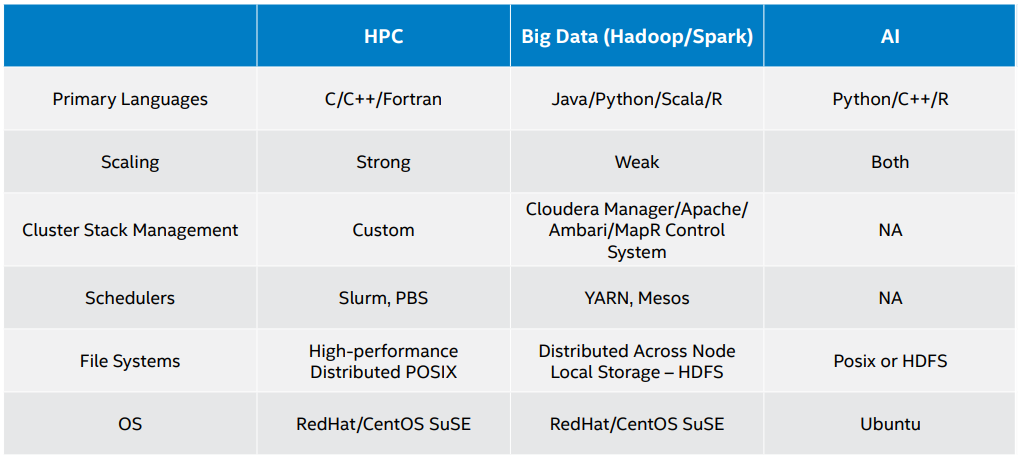
\includegraphics[width=\linewidth]{images/hpc-bigdata-ai-envs.png}
    \caption{HPC与AI、Big Data的软件环境对比\cite{bring_ai_to_hpc}}
    \label{hpc_bigdata_ai_envs}
\end{figure}

在科研领域已经有开源的\href{https://ophidia.cmcc.it/}{Ophidia}\;HPDA框架,
尝试将HPC和Big Data结合起来,解决eScience领域的大数据问题。
它的整体架构如\cref{ophidia_arch}所示\cite{hpda_escience}。

\begin{figure}[ht!]
    \centering
    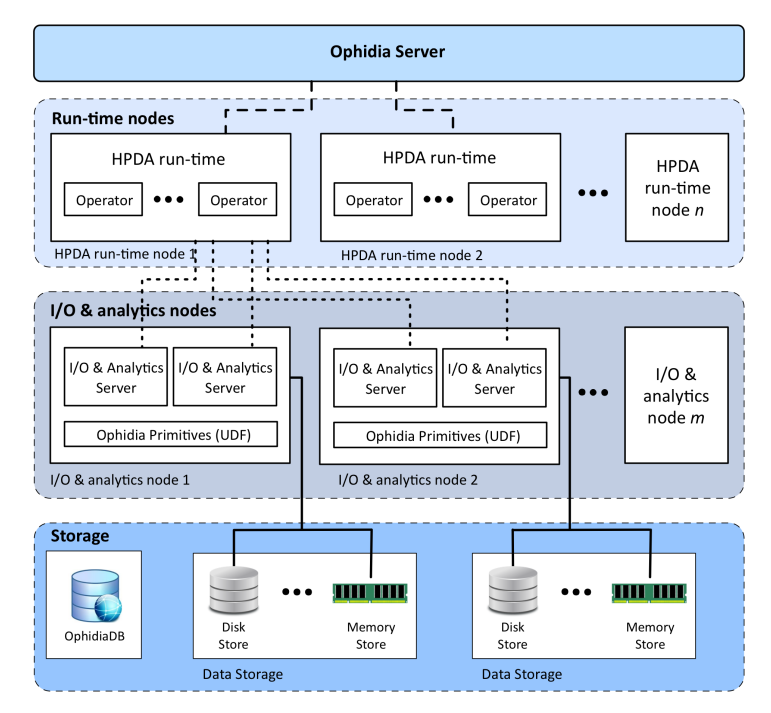
\includegraphics[width=\linewidth]{images/ophidia_hpda_arch.png}
    \caption{Ophidia HPDA框架的顶层架构}
    \label{ophidia_arch}
\end{figure}

\subsection{HPDA与serverless}

应用HPDA需要各种各样的编程环境和运行时,
为了进行性能调优可能还需要内嵌调试信息,
计算负载如何能够随时随地执行(尤其是虚拟化环境中),
是一个关键问题。一种思路是将各个资源内嵌到工作负载的编译产物中,
但是这样会带来很多无关代码、增大执行程序体积;
另一种方式则是屏蔽掉底层细节,
使用容器、甚至serverless/FaaS模式。

以容器化为代表的虚拟化技术发展如今已经十分成熟(参见\cref{virtualization}),
在应用领域已经应用十分广泛。
利用容器化技术,可以将HPDA运行时进行封装,
从而能够更容易进行部署和伸缩,
极大提高应用的可移植性。
例如NVIDIA提供AI/HPC容器\footnote{见:https://developer.nvidia.com/ai-hpc-containers},
每月更新提供更佳的性能优化。
而FaaS能更好地提供逻辑抽象、数据模型等,
因此有望作为更流畅的HPC运行时\cite{hpc_future}。

\begin{figure}[ht!]
    \centering
    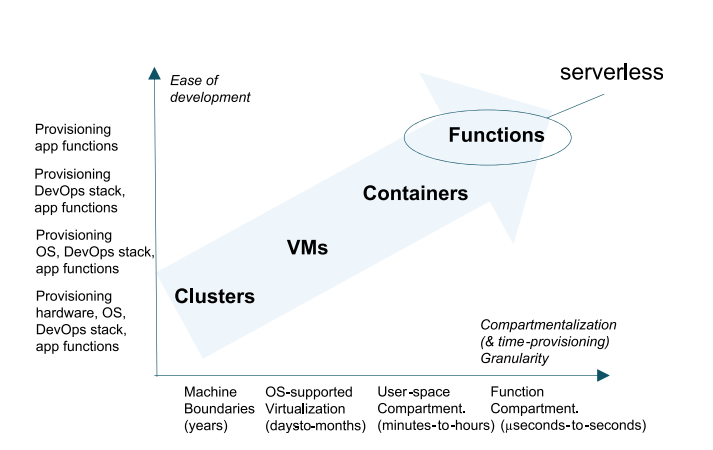
\includegraphics[width=\linewidth]{images/evolution-of-virtualization.png}
    \caption{虚拟化技术的演进\cite{hpc_future}}
    \label{virtualization}
\end{figure}